 \documentclass[a4paper,14pt]{report} %размер бумаги устанавливаем А4, шрифт 14пунктов
 \usepackage{kmanual} % мой стиль
        
%\includeonly{Title_ag, other_ag}
 \makeatletter

 \makeatother

 % колонтитулы:
 \pagestyle{fancy}
  \fancyhead{} %очистим хидер на всякий случай
  \fancyfoot{} %очистим футер 
  \renewcommand{\sectionmark}[1]{\protect\markright{\textit{#1}}}
  \fancyfoot[R]{\thepage} %номер страницы справа внизу
  \fancyhead[R]{\parbox[b]{200pt}{\flushright{\textbf{\textit{Система администрирования ЛПУ}}}}}
  \fancyhead[L]{
\includegraphics[width = 150pt, keepaspectratio]{korus}}
  \fancyfoot[L]{\textit{Руководство администратора} \\ \rightmark} 
  \renewcommand{\headrulewidth}{0.3pt}
  \renewcommand{\footrulewidth}{0.3pt}
  \addtolength{\headheight}{0.3pt} % оставляем место для линейки
  \fancypagestyle{plain}

 \fancypagestyle{firststyle} %стиль первой страницы
 {
  \fancyhead{} %очистим хидер на всякий случай
  \fancyfoot{} %очистим футер 
  \fancyhead[R]{\parbox[b]{200pt}{\flushright{\textbf{\textit{Система администирования ЛПУ}}}}}
  \fancyhead[L]{
\includegraphics[width = 150pt, keepaspectratio]{korus}}
  \renewcommand{\headrulewidth}{0.3pt}
  \renewcommand{\footrulewidth}{0pt}
  \addtolength{\headheight}{0.3pt} % оставляем место для линейки
 }
  
 \begin{document}
   
   \begin{titlepage}
    \newpage
    \thispagestyle{firststyle} %стиль колонтитулов
    
    \begin{center}
    \vspace*{\fill}
    \hbox{%
    \vrule width 4pt\hspace{2em}\parbox{1\textwidth}%
    {\vspace*{0.5em}\raggedright{\Large{\textbf{СИСТЕМА АДМИНИСТРИРОВАНИЯ ЛПУ}}}

    \vspace*{1em}
    \Large{\textbf{РУКОВОДСТВО ПОЛЬЗОВАТЕЛЯ}}
    }}
    \end{center}

    \vspace{\fill}

    \begin{flushleft}
    Дата создания:  30.11.13 \\
 %   \vspace{1em}
    Последнее обновление:  30.11.13\\
 %   \vspace{1em}
    Версия:  1.0\\
    \end{flushleft}
    \clearpage
    \end{titlepage}%титульный лист
  \tableofcontents % оглавление, которое генерируется автоматически
  \newpage
\sect{Введение}

 Настоящий документ предназначен для персонала медицинского учреждения, ответственного за выгрузку данных в ТФОМС, работников отделов информатизации и автоматизации.
 
 Данное руководство пользователя содержит все необходимые сведения для организации работы по выгрузке и загрузке данных в ТФОМС.
 
 Для работы в Системе администрирования ЛПУ и понимания материала настоящего документа сотрудник должен владеть основной терминологией пользователя ПК, иметь навыки работы на компьютере не ниже уровня пользователя ПК.
 
 Система администрирования ЛПУ – это информационная система 
 

\newpage
\sect{Назначение и условия применения}

 Руководство пользователя является основным справочным документом пользователя по работе с системой. Оно может быть использовано как для обучения работе в системе новых пользователей, так и для расширения и закрепления знаний и навыков пользователей, имеющих опыт работы в системе администрирования ЛПУ.
 
 При возникновении проблем во время работы с Системой администрирования ЛПУ, пользователь должен, в первую очередь, прибегнуть к настоящему документу для поиска решения проблемы, и только в случае, если с помощью данного документа проблему разрешить не удалось, обратиться в службу технической поддержки.
 
 В документе будут использоваться следующие условные обозначения:  \vspace*{0.5em}
 
 \dm{Название} -- так в тексте будут выделяться название полей и пунктов меню приложения.
 
 \btn{OK} -- так будут обозначаться кнопки экранных форм.
 
 \keys{F1} -- так будут обозначаться клавиши на клавиатуре.
 
 \begin{vnim}
  Так будут обозначаться важные предупреждения. Их необходимо прочесть перед выполнением дальнейших инструкций!
 \end{vnim}
 
 \begin{prim}
 Так будут обозначаться полезные замечания, которые не являются обязательными для изучения, однако могут значительно повысить эффективность работы. Продвинутым пользователям рекомендуется обратить на них внимание.
 \end{prim}
 %введение и прочая вводная часть
  \newpage
\section{Общие сведения о системе}

\subsection{Вход в систему}

Перед началом работы в системе необходимо получить персональный идентификатор пользователя (логин) и пароль у администратора.

\begin{vnim}
 Персональный идентификатор и пароль предназначены для индивидуального доступа в систему. Никогда не сообщайте их третьим лицам!
\end{vnim}
 
Для того чтобы начать работать с Системой администрирования ЛПУ, необходимо войти в нее, используя персональный идентификатор и пароль. Процедура входа в систему называется \dm{авторизацией}. \label{auth}

\begin{figure}[ht]\centering
 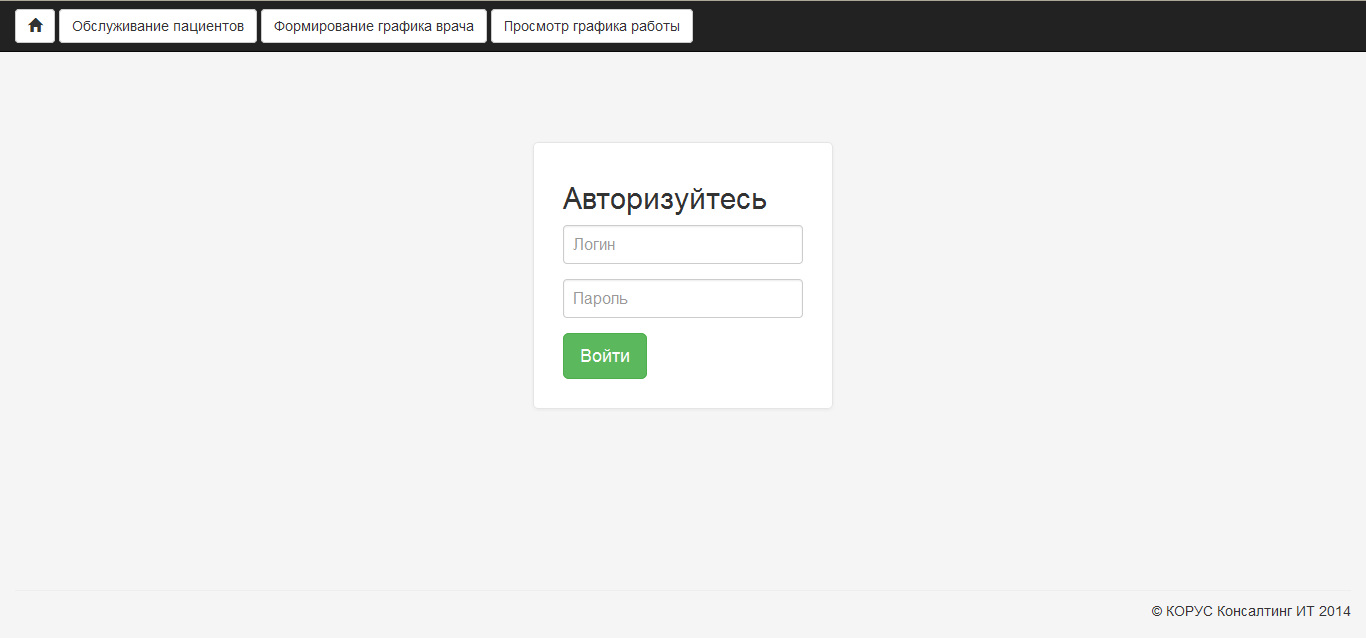
\includegraphics[width = 1\textwidth ,keepaspectratio]{gen_login}
 \caption{Форма авторизации пользователя}
 \label{img_gen_login}
\end{figure} 

Доступ к системе можно получить следующими способами:
\begin{itemize}
 \item Запустить приложение с помощью ярлыка на рабочем столе.
 \item Открыть любой из доступных Web-браузеров (Internet Explore, Firefox, Opera, Chrome и др.) и в адресной строке ввести адрес сервера, полученный у администратора системы.
\end{itemize}

После выполнения любого из описанных действий откроется форма авторизации (Рисунок \ref{img_gen_login}), где следует ввести идентификатор пользователя, пароль и нажать кнопку \btn{Войти}.

В случае успешной авторизации откроется главная страница системы (Рисунок \ref{img_gen_main}).

\begin{figure}[ht]\centering
 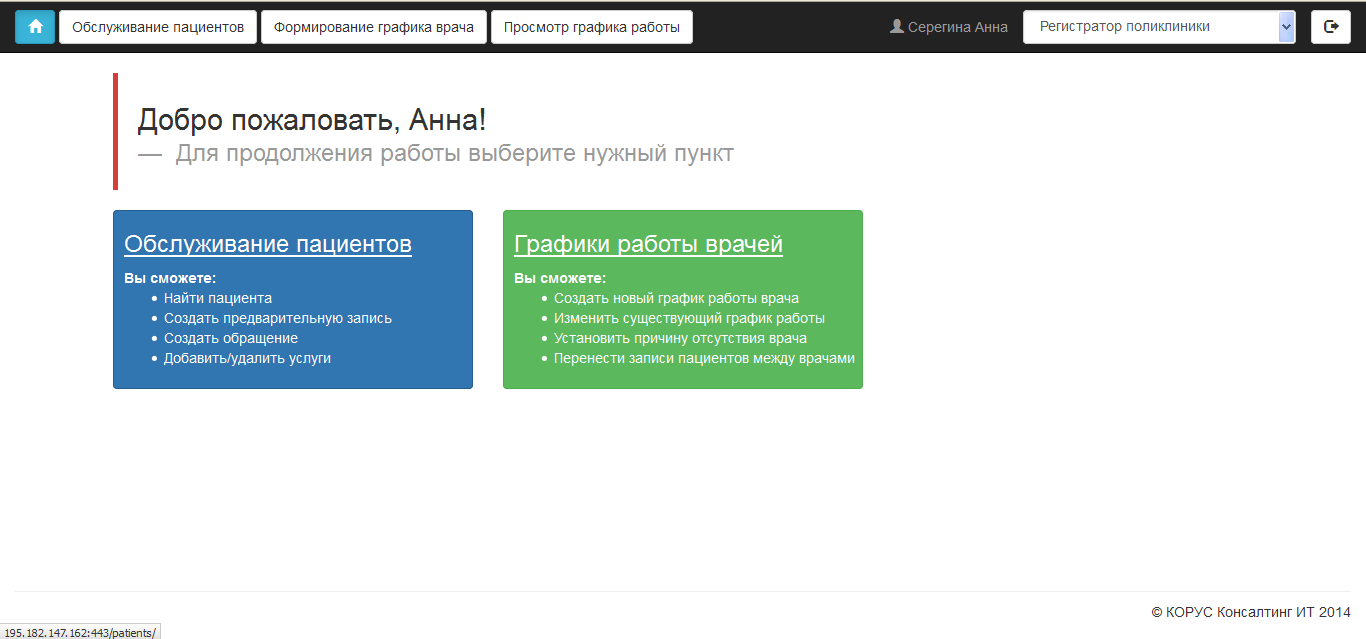
\includegraphics[width = 1\textwidth ,keepaspectratio]{gen_main}
 \caption{Главная страница системы}
 \label{img_gen_main}
\end{figure} 

Если в процессе авторизации возникла какая-либо ошибка, сообщение появится над полем для ввода логина (Рисунок \ref{img_gen_lfail}).

В случае возникновения ошибки «Неверная пара логин/пароль» необходимо:
\begin{enumerate}
 \item Проверить правильность введенного идентификатора пользователя;
 \item Проверить правильность введенного адреса для подключения (если вводился вручную);
 \item Проверить язык ввода;
 \item Проверить состояние клавиши \keys{CapsLock} на клавиатуре и выключить ее при необходимости;
 \item Если в пароле присутствуют цифры, проверить состояние клавиши \keys{NumLock}, включить ее при необходимости;
 \item Повторить попытку авторизации.
\end{enumerate}
 
Если проблема не была решена, нужно обратиться к администратору системы для проверки идентификационных данных.

\begin{figure}[ht]\centering
 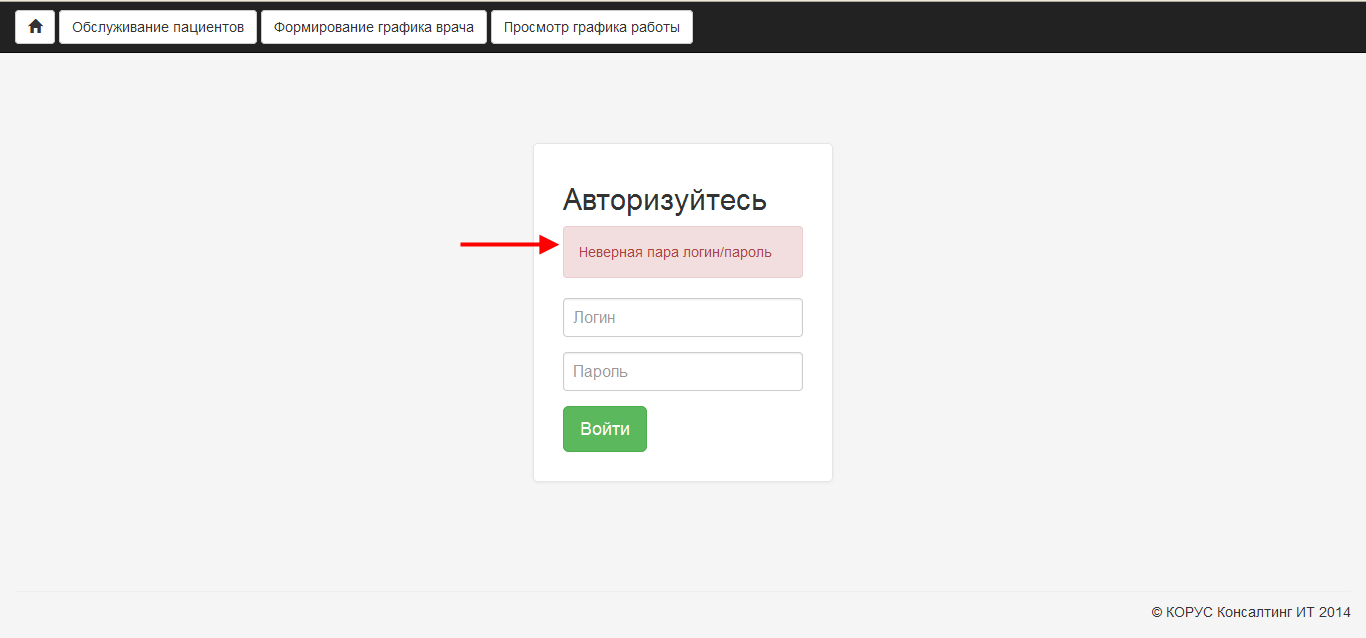
\includegraphics[width = 1\textwidth ,keepaspectratio]{gen_lfail}
 \caption{Ошибка авторизации}
 \label{img_gen_lfail}
\end{figure} 

\subsection{Завершение работы}

После завершения работы, необходимо выйти из системы. Для этого нужно нажать кнопку 
\includegraphics{exit} в правом верхнем углу страницы. Будет осуществлен выход из системы и возврат на страницу авторизации. Если требуется войти в систему под другим именем пользователя, следует пройти процедуру авторизации с новыми идентификационными данными. Если работа с системой завершена, можно закрыть Web-браузер, нажав на кнопку \btn{x} в правом верхнем углу окна или выбрав в главном меню пункт \mm{Файл \str Выход}.

\subsection{Основные принципы работы}

Система администрирования ЛПУ (или система) работает через Web-интерфейс и не требует установки на клиентской рабочей станции никакого дополнительного программного обеспечения. Единственным обязательным условием является наличие установленного Web-браузера, который, как правило, включен по умолчанию при установке любой операционной системы.

Вся работа в системе производится в окне Web-браузера. В верхней части каждой страницы находится панель управления (Рисунок \ref{img_gen_main}).

В левой ее части находятся список доступных подсистем. При нажатии на кнопку с названием подсистемы осуществляется переход на главную страницу выбранной подсистемы. При нажатии на кнопку 
\includegraphics{home} выполняется переход на главную страницу системы.

В правой части панели управления находятся следующие кнопки:
\begin{itemize}
 \item Кнопка 
\includegraphics{help}  вызывает справку по основным управляющим элементам текущей страницы.
 \item Кнопка 
\includegraphics{exit}  позволяет выйти из системы.
\end{itemize}

\begin{prim}
 После авторизации в системе возможно одновременное открытие нескольких страниц системы. Страницы могут быть открыты в отдельных окнах или вкладках. Для открытия страницы в новой вкладке или новом окне можно воспользоваться контекстным меню или колесом прокрутки мыши.
\end{prim}

\subsubsection{Работа со справкой}

Кнопка 
\includegraphics{help}  находится на панели управления в правом верхнем углу любой страницы Системы администрирования ЛПУ. При нажатии на нее появляется окно подсказки, последовательно описывающее назначение основных управляющих элементов страницы (Рисунок \ref{img_gen_help}).

\begin{figure}[ht]\centering
 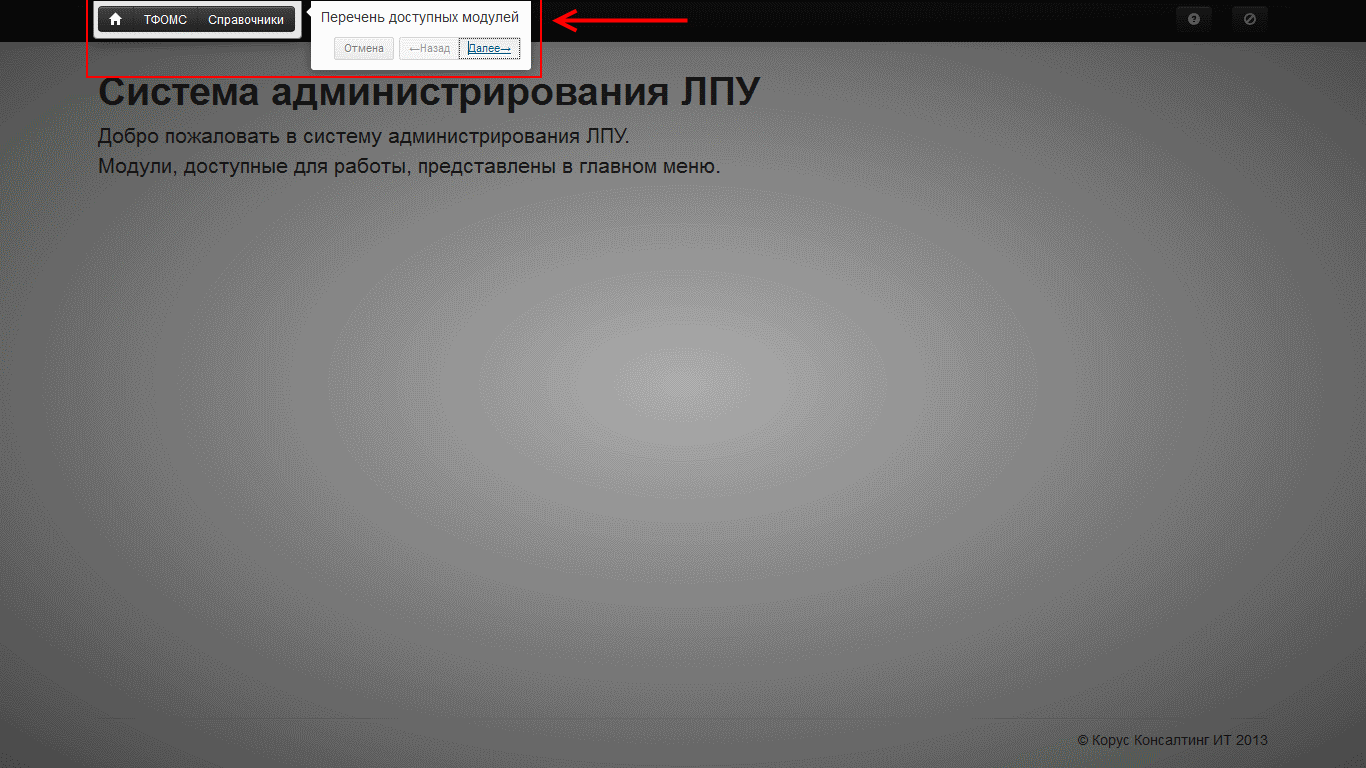
\includegraphics[width = 1\textwidth ,keepaspectratio]{gen_help}
 \caption{Справка по панели управления}
 \label{img_gen_help}
\end{figure} 

Для перехода к следующему элементу необходимо нажать кнопку \btn{Далее $\to$}  в окне подсказки или клавишу \keys{$\to$} на клавиатуре. Окно подсказки переместится к следующему управляющему элементу страницы и отобразит подсказку по нему. Если был достигнут последний управляющий элемент страницы, то окно подсказки закрывается.

Для возврата к предыдущему управляющему элементу нужно нажать кнопку \btn{$\gets$ Назад}  или клавишу \keys{$\gets$} на клавиатуре.

При нажатии на кнопку \btn{Отмена} окно подсказки закрывается.
 %общие сведения о системе
  \newpage
\section{Подсистема журналирования}

Система журналирования – это внешний модуль, позволяющий вести лог следующих событий в ФТМИС:
\begin{itemize}
 \item Авторизация пользователя в системе;
 \item Печать документа;
 \item Cоздание, удаление, изменение типов действий;
 \item Создание, удаление, изменение событий;
 \item Создание, удаление, изменение действий;
 \item Ошибки, связанные с ошибками работы, обращениями в БД.
\end{itemize}

\begin{figure}[ht]\centering
 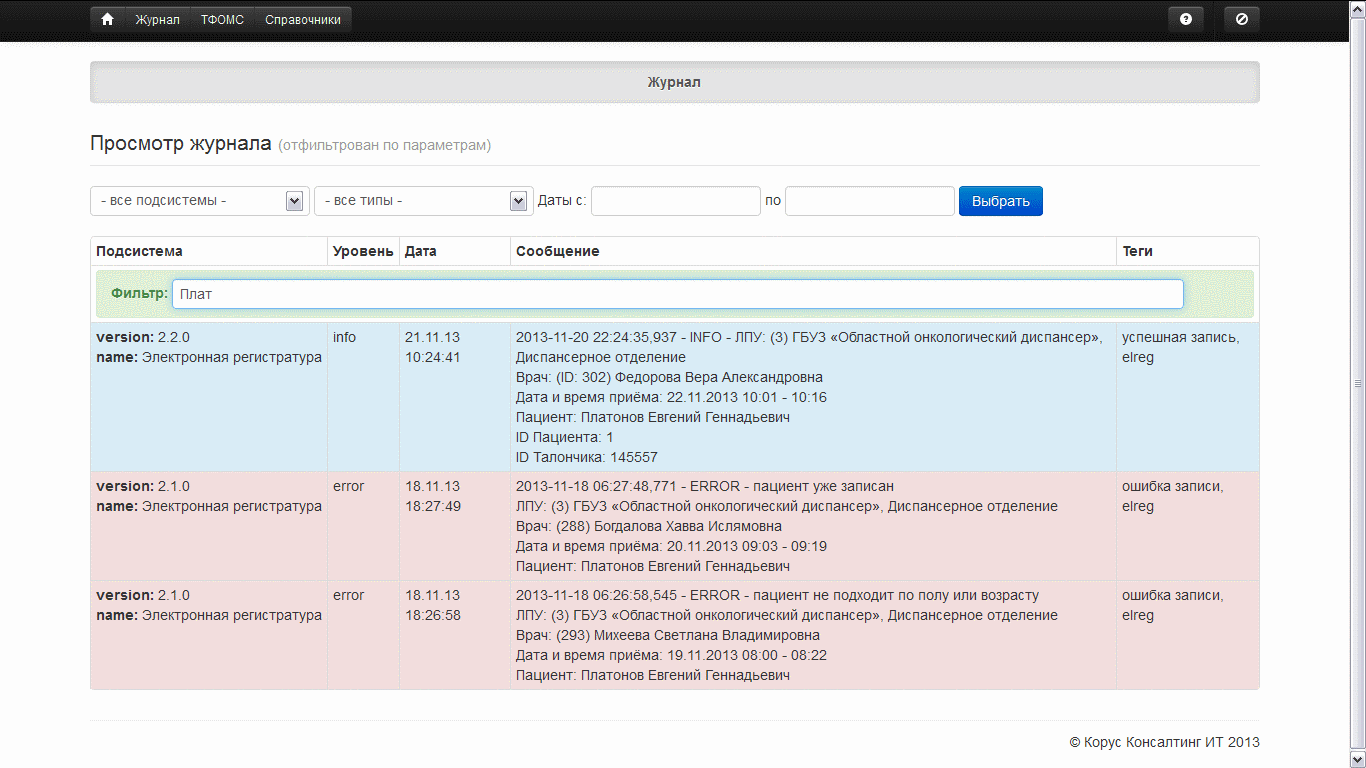
\includegraphics[width = 1\textwidth ,keepaspectratio]{log_jur}
 \caption{Журнал событий}
 \label{img_log_jur}
\end{figure} 
 
Для ведения лога необходимо, чтобы журналирование событий было включено на стороне ФТМИС.

Система администрирования ЛПУ позволяет просматривать описанный выше лог в удобном виде, дает возможность фильтровать события по различным параметрам.

Для перехода к просмотру журнала событий необходимо нажать кнопку \btn{Журнал} на панели управления. Будет осуществлен переход на страницу просмотра журнала (Рисунок \ref{img_log_jur}).

По умолчанию отображаются последние 100 записей лога событий. Данные представлены в виде таблицы, имеющей следующие столбцы:
\begin{itemize}
 \item В столбце \dm{Подсистема} представлена информация о рабочей станции и пользователе, инициировавшем событие. Указывается IP-адрес рабочей станции (\dm{IP}), название рабочей станции/имя компьютера (\dm{host}), версия клиентской части ФТМИС, с помощью которой было совершено данное событие (\dm{version}) и имя пользователя, под которым был осуществлен вход в ФТМИС (\dm{user}).
 \item В столбце \dm{Уровень} указывается уровень значимости сообщения. Выделяются следующие уровни (от наиболее важного к наименее значимому):
 \begin{itemize}
  \item Critical – критические ошибки, возникающая в процессе работы или при обращении к базе данных.
  \item Error – ошибка, возникающая в процессе работы или при обращении к базе данных. Записи данного типа окрашены в розовый цвет.
  \item Warning – предупреждения, возникающая в процессе работы или при обращении к базе данных.
  \item Notice – записи лога об успешно совершенных событиях. К данной группе относятся записи о совершении входа в систему, печати документов, создании, изменении, удалении типов действий и событий. Записи данного типа окрашены в голубой цвет.
  \item Note – аналогично предыдущему, запись лога о совершенных стандартных событиях. В данной группе относятся данные о записи пациентов на прием, создании, изменении, удалении действий. Записи данного типа окрашены в голубой цвет.
  \item Debug – сообщения, используемые для отладки работы системы (разработчиками). Записи данного типа окрашены в белый цвет.
 \end{itemize}
 \item В столбце \dm{Дата} указывается дата и время совершения указанного события. Время может браться с сервера системы журналирования либо из ФТМИС в зависимости от настроек.
 \item В столбце \dm{Сообщение} отображается краткая информация о совершенном событии. Как правило, в поле содержится название события, идентификатор и фамилия пациента, медицинские записи которого подвергались обработке. Состав информации в данном поле определяется типом информационного сообщения. Например, сообщение о входе пользователя в систему содержит только название, а сообщение о записи пациента на прием содержит код и название ЛПУ и фамилию врача, к которому записывается пациент; дату и время, на которые осуществлена запись; идентификатор и фамилию пациента, а так же идентификатор выданного талона. Для событий уровня critical или error в данном поле может содержаться текст ошибки.
 \item В столбце \dm{Теги} указываются основные ключевые слова для данного события. Теги привязаны к виду события. Соответственно, события одного вида имеют одни и те же теги.
\end{itemize}
 
Для отбора записей лога по определенным параметрам можно воспользоваться фильтром. Фильтр предусмотрен по полям: \dm{Подсистема}, \dm{Уровень}, \dm{Дата}.

В поле \dm{Подсистема} можно выбрать определенное сочетание (рабочая станция – имя пользователя). Тогда после применения фильтра будут отображаться только события совершенные выбранным пользователем с выбранной рабочей станции.

В следующем поле можно выбрать уровень события (critical, error, warning, notice, note, debug). Если в поле ничего не выбрано, то в таблице отображаются события всех уровней.

В полях \dm{Дата с} \dm{по} указываются даты начала и окончания периода, за который необходимо отобразить лог событий. Дату можно выбрать из календаря или ввести с клавиатуры. Календарь раскрывается при установке курсора в поле для ввода даты.

После того как параметры фильтра установлены, необходимо нажать кнопку \btn{Выбрать} справа от полей задания параметров фильтрации. Данные лога событий будут отфильтрованы в соответствии с указанными параметрами.

Ниже находится еще одна строка, с помощью которой можно фильтровать данные – поле \dm{Фильтр}. Но если фильтр, описанный ранее (далее основной фильтр), позволяет выбрать любые данные из лога согласно параметрам фильтрации, то строка \dm{Фильтр} (или строка фильтрации) позволяет выбирать данные только среди записей, отображенных на экране на момент ввода данных в строку фильтрации. Фильтрация записей в таблице происходит автоматически по мере ввода данных в строку \dm{Фильтр}. В результат фильтрации попадут записи, в любой из ячеек которых встречается буквосочетание, введенное в строку фильтрации. Для снятия данного фильтра достаточно очистить поле \dm{Фильтр}. Тогда на экране снова будут отображаться записи, выбранные с помощью основного фильтра.
 %Подсистема журналирования
  \newpage
\section{Подсистема выгрузки в ТФОМС}

Подсистема выгрузки в ТФОМС позволяет:
\begin{itemize}
 \item выгружать из ФТМИС данные о пролеченных пациентах для последующей отправки в ТФОМС;
 \item выгружать из ФТМИС данные об обращениях пациентов для последующей отправки в ТФОМС;
 \item загружать ответы от ТФОМС о принятых или отклоненных случаях обращения;
 \item хранить и просматривать отчеты о выполненных операциях.
\end{itemize}
 
Система позволяет осуществлять выгрузку в форматах:
\begin{itemize}
 \item XML;
 \item DBF.
\end{itemize}
 
Загрузка ответов от ТФОМС осуществляется только в формате XML.

Выгрузка данных осуществляется по заранее настроенным шаблонам выгрузки. Настройку шаблонов выполняет администратор системы.

При переходе в подсистему выгрузки в ТФОМС открывается главная страница подсистемы (Рисунок \ref{img_tfoms_main}). В верхней части страницы расположены кнопки перехода в соответствующий раздел. Переход в раздел \dm{Выгрузка} так же осуществляется при нажатии кнопок \btn{Cформировать реестры} или \btn{Перейти к выгрузке >>}  на главной странице подсистемы. Переход в раздел \dm{Загрузка} так же осуществляется при нажатии кнопки \btn{Загрузить из ТФОИМС >>}.  

\begin{figure}[ht]\centering
 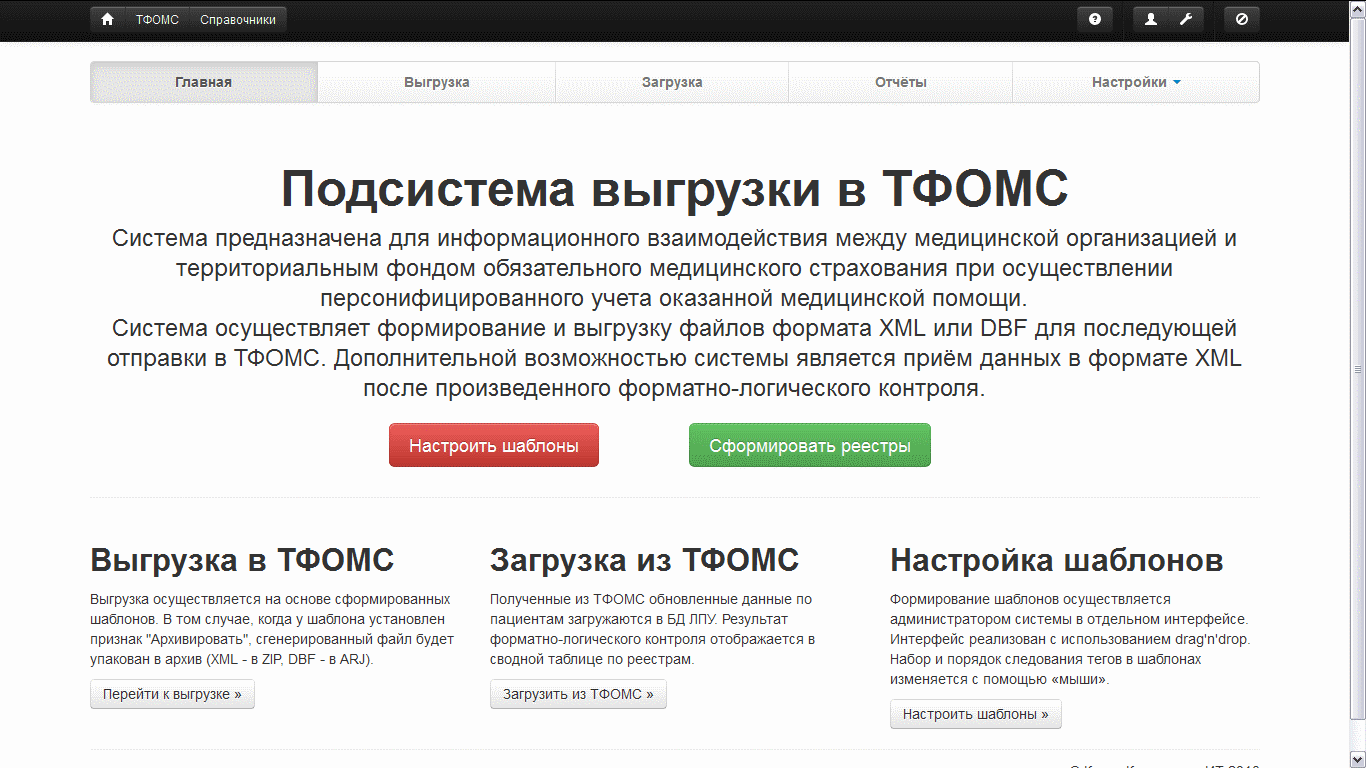
\includegraphics[width = 1\textwidth ,keepaspectratio]{tfoms_main}
 \caption{Главная страница подсистемы выгрузки в ТФОМС}
 \label{img_tfoms_main}
\end{figure} 

\subsection{Выгрузка}

В данном разделе подсистемы осуществляется выгрузка данных о пролеченных пациентах и их обращениях для последующей передачи в ТФОМС.

Для перехода в данный раздел (Рисунок \ref{img_tfoms_unload}) необходимо нажать кнопку \btn{Выгрузка} в верхней части любой страницы подсистемы либо нажать кнопку \btn{Cформировать реестры}  или \btn{Перейти к выгрузке}  на главной странице подсистемы.

\begin{figure}[ht]\centering
 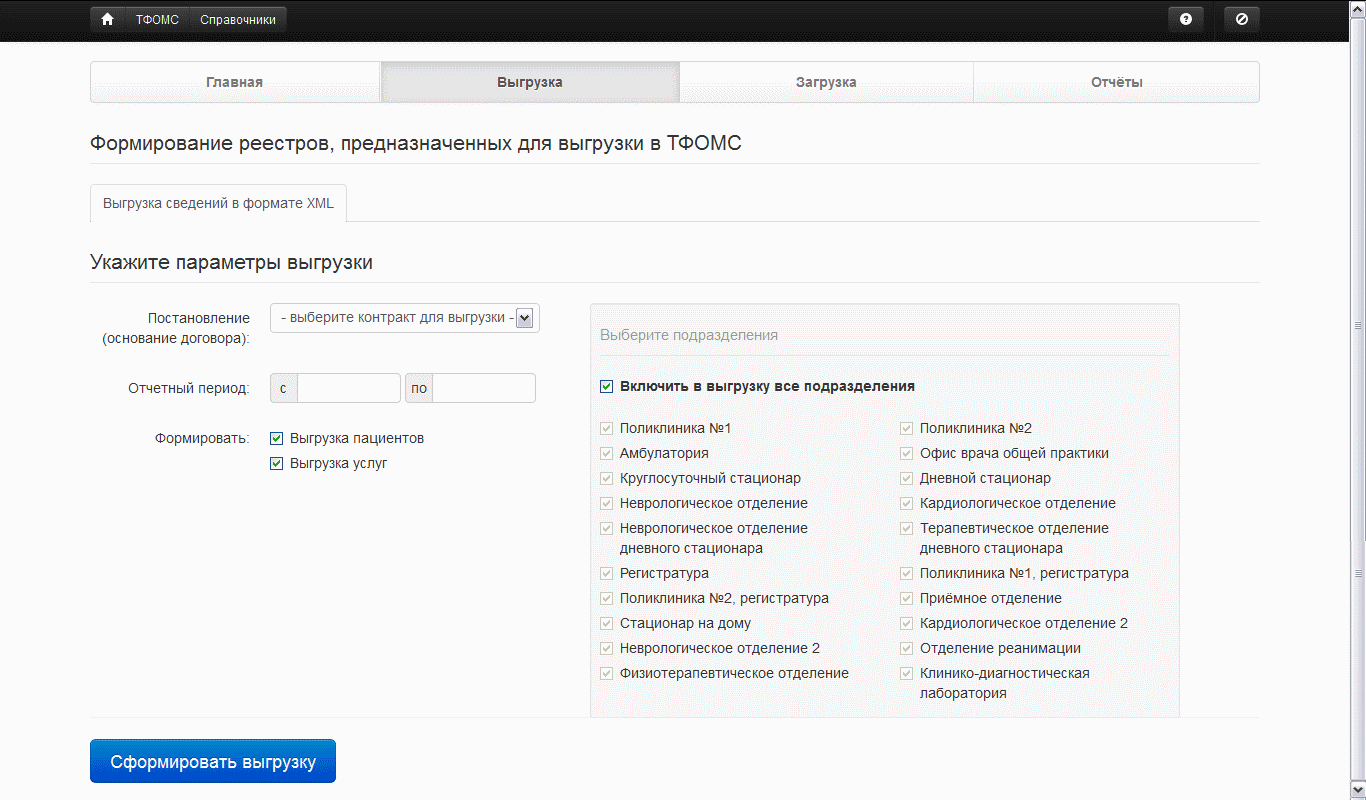
\includegraphics[width = 1\textwidth ,keepaspectratio]{tfoms_unload}
 \caption{Раздел <<Выгрузка>> подсистемы выгрузки в ТФОМС}
 \label{img_tfoms_unload}
\end{figure}

Для осуществления выгрузки необходимо:
\begin{enumerate}
 \item Выбрать вкладку, соответствующую требуемому формату выгрузки.
 \item Указать параметры выгрузки (см. ниже).
 \item Нажать кнопку \btn{Сформировать выгрузку}.
\end{enumerate}

При выгрузке задаются следующие параметры:
\begin{itemize}
 \item \dm{Постановление (основание договора)} – выбирается из списка основание договора (источник финансирования), по которому будет осуществляться выгрузка.
 item \dm{Отчетный период} – период, за который следует выгружать данные о случаях обращения. Указываются начальная и конечная дата периода. Даты заполняются вручную с клавиатуры или выбираются из календаря. Календарь раскрывается автоматически при установке курсора в поле даты.
 \item При установке флажка \dm{Выгрузка пациентов} будет осуществляться выгрузка персональных данных пациентов, получивших медицинскую помощь в указанный период.
 \item При установке флажка \dm{Выгрузка услуг} будет осуществляться выгрузка сведений о случаях обращений пациентов за медицинской помощью в указанный период.
 \item В блоке выбора подразделения можно выбрать отдельные отделения, по которым необходимо выполнить выгрузку. При установке флажка \dm{Включить в выгрузку все подразделения}, флажки устанавливаются автоматически для всех перечисленных подразделений, а редактирование их становится невозможным. Для того чтобы снова иметь возможность выбора подразделений, следует снять флажок \dm{Включить в выгрузку все подразделения}.
\end{itemize}
 
Формирование выгрузки может занять продолжительное время. Во время подготовки данных на экране будет отображаться страница ожидания (Рисунок \ref{img_tfoms_unload_proc}).

\begin{figure}[ht]\centering
 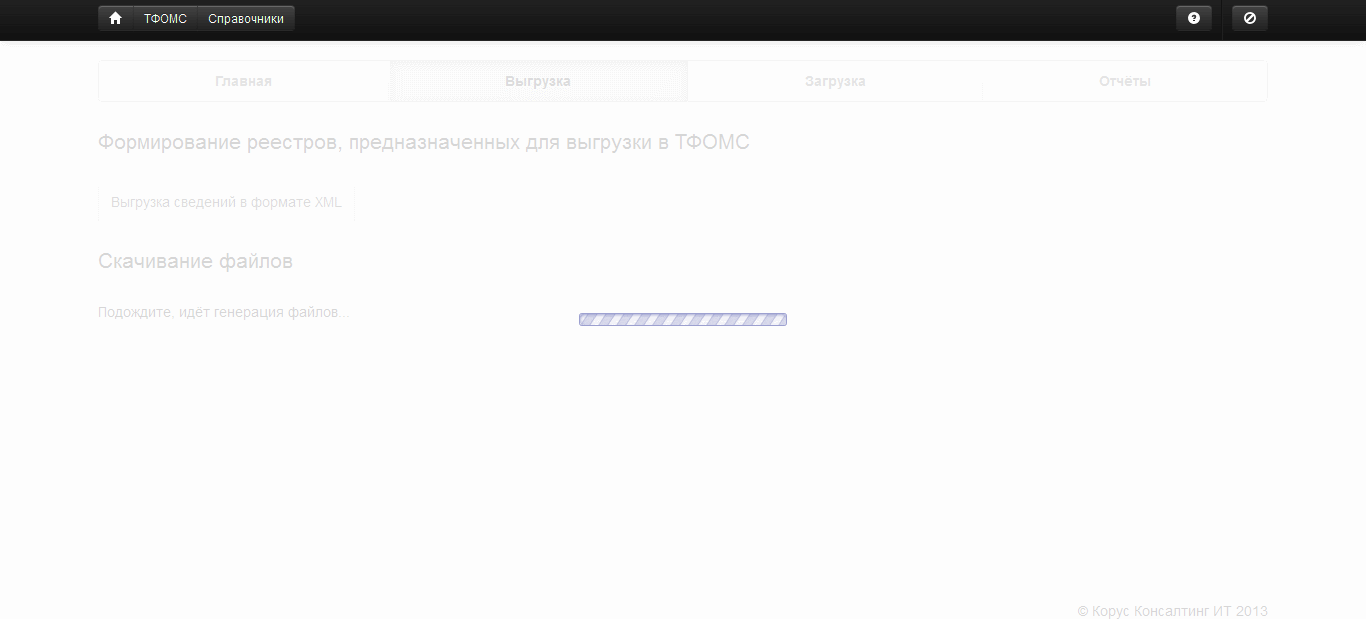
\includegraphics[width = 1\textwidth ,keepaspectratio]{tfoms_unload_proc}
 \caption{Выполнение выгрузки}
 \label{img_tfoms_unload_proc}
\end{figure}

После того как файлы выгрузки будут сформированы, они станут доступны для скачивания. Для скачивания файла необходимо щелкнуть по нему левой кнопкой мыши, в появившемся окне выбрать Сохранить и нажать кнопку \btn{OK}, а затем указать папку для сохранения.

В зависимости от настроек шаблона выгрузки файлы могут быть выгружены в заархивированном (ZIP, ARJ) или распакованном виде.

\subsection{Загрузка}

В данном разделе подсистемы осуществляется загрузка данных об отклоненных случаях обращений по результатам проверки в ТФОМС для ранее выгруженных данных.

\begin{vnim}
 Загрузка данных возможна только в формате XML
\end{vnim}

Для перехода в данный раздел (Рисунок \ref{img_tfoms_upload}) необходимо нажать кнопку \btn{Звгрузка}  в верхней части любой страницы подсистемы либо нажать кнопку \btn{Загрузить из ТФОМС >>}  на главной странице подсистемы.

\begin{figure}[ht]\centering
 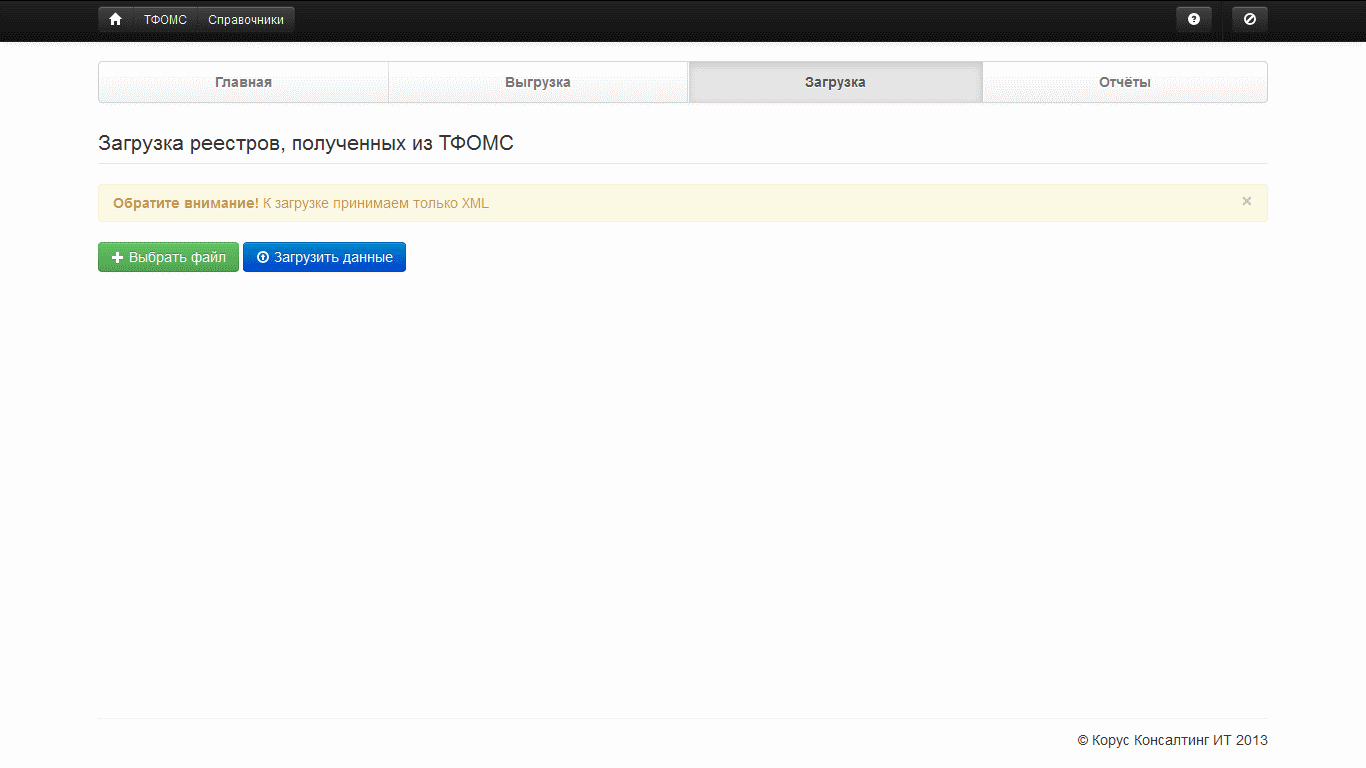
\includegraphics[width = 1\textwidth ,keepaspectratio]{tfoms_upload}
 \caption{Раздел <<Загрузка>> подсистемы выгрузки в ТФОМС}
 \label{img_tfoms_upload}
\end{figure}

Для загрузки результатов проверки ранее выгруженных файлов необходимо нажать на кнопку \btn{Выбрать файл}, в открывшемся окне перейти в нужную папку и выбрать файл для загрузки. После выбора файла его имя появится под кнопкой \btn{Выбрать файл}. Далее необходимо нажать кнопку \btn{Загрузить данные}. После непродолжительного ожидания на странице появится сообщение о результатах загрузки (Рисунок \ref{img_tfoms_upload_rez}).

\begin{figure}[ht]\centering
 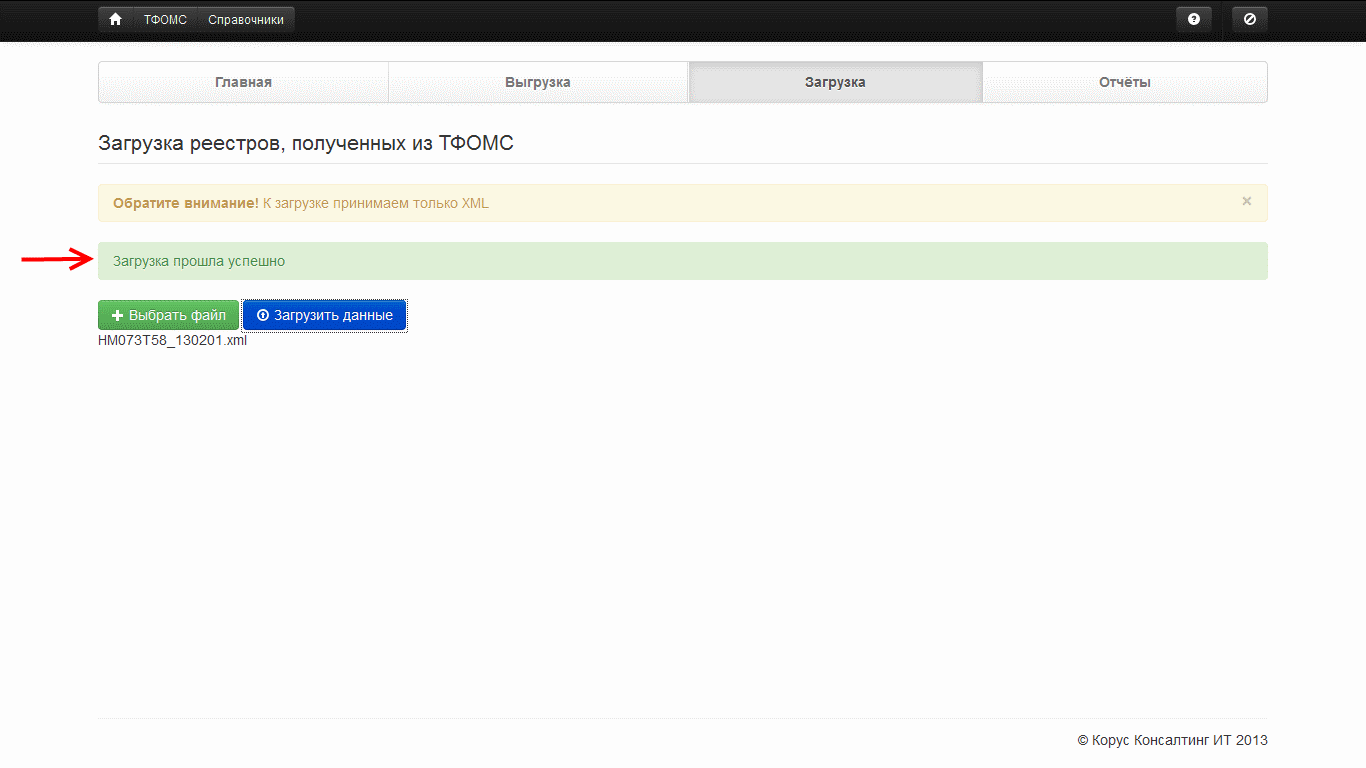
\includegraphics[width = 1\textwidth ,keepaspectratio]{tfoms_upload_rez}
 \caption{Результат загрузки файла}
 \label{img_tfoms_upload_rez}
\end{figure}

\subsection{Отчеты}

В разделе \dm{Отчеты} хранится история выполненных выгрузок. По любой из выгрузок можно просмотреть позиции, попавшие в счет и повторно скачать файлы, полученные в результате выгрузки.

Для перехода в данный раздел (Рисунок \ref{img_tfoms_rep}) необходимо нажать кнопку \btn{Отчеты}  в верхней части любой страницы подсистемы. Список всех выгрузок в ТФОМС будет представлен в виде таблицы.

\begin{figure}[ht]\centering
 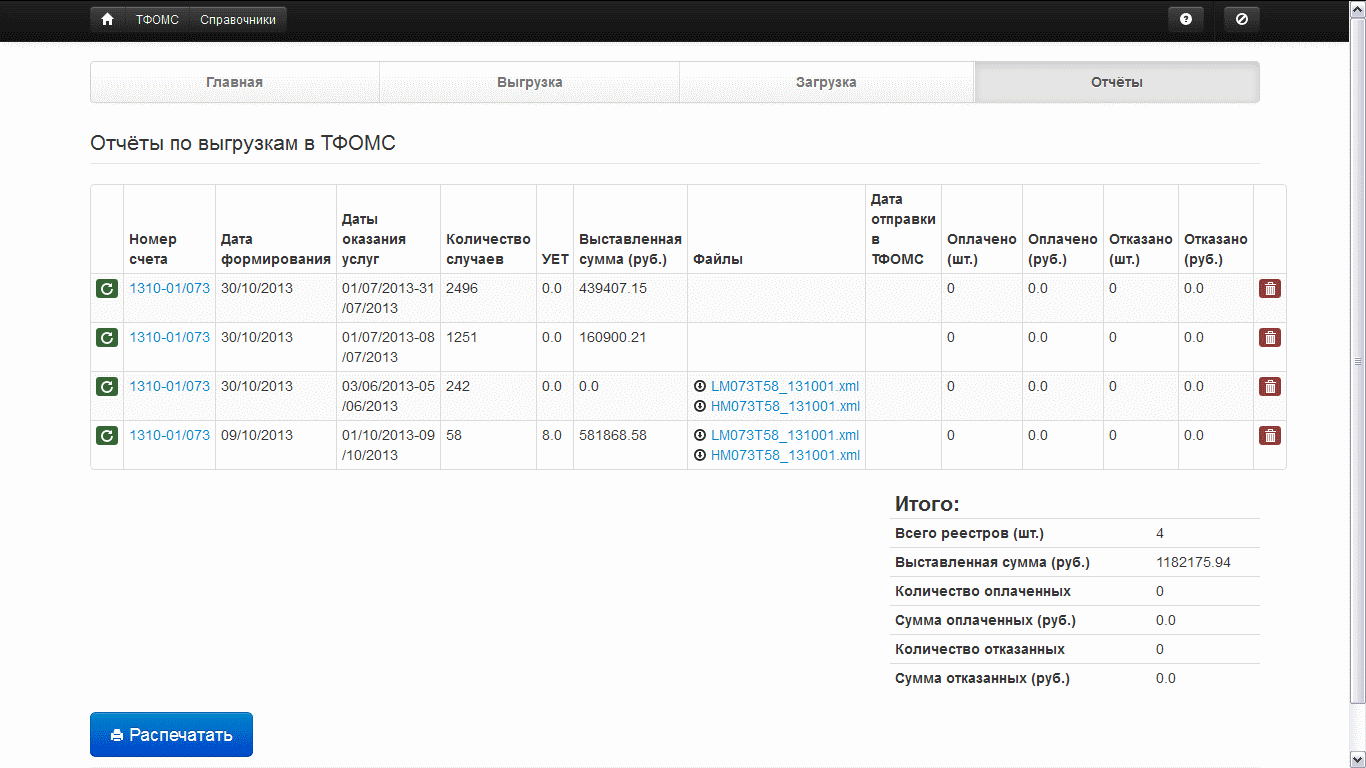
\includegraphics[width = 1\textwidth ,keepaspectratio]{tfoms_rep}
 \caption{Раздел <<Отчеты>> подсистемы выгрузки в ТФОМС}
 \label{img_tfoms_rep}
\end{figure}

Кнопка 
\includegraphics{re} позволяет сформировать выбранную выгрузку еще раз. При ее нажатии осуществляется автоматический переход в раздел \dm{Выгрузки}, а параметры выгрузки устанавливаются такими же, как при текущей выгрузке. При необходимости можно изменить параметры. Для запуска повторной выгрузки следует нажать кнопку \btn{Сяормировать выгрузку}. После ее завершения в список отчетов добавится новая строка.

Кнопка 
\includegraphics{del}  позволяет удалить выбранный отчет. После нажатия на нее необходимо подтвердить удаление в появившемся окне (Рисунок \ref{img_tfoms_rep_del}).

\begin{figure}[ht]\centering
 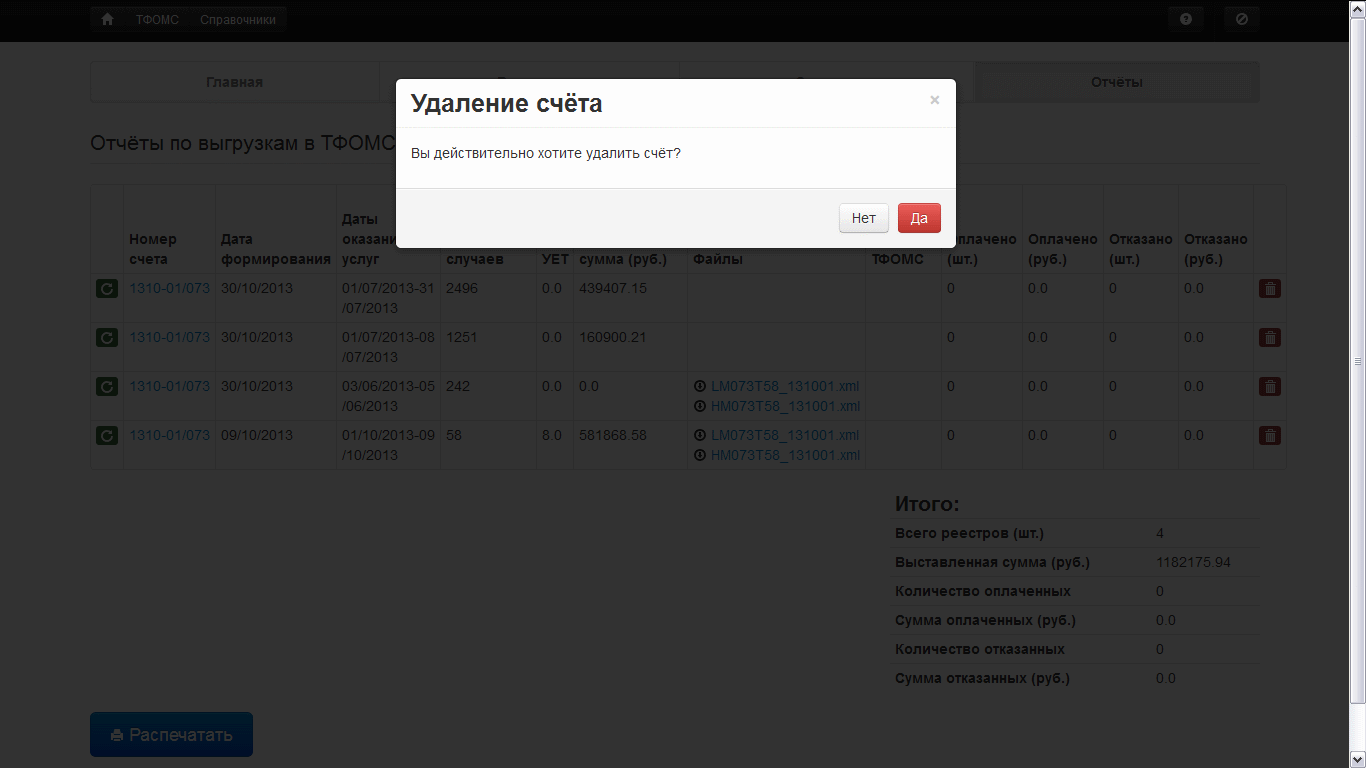
\includegraphics[width = 1\textwidth ,keepaspectratio]{tfoms_rep_del}
 \caption{Подтверждение удаления отчета}
 \label{img_tfoms_rep_del}
\end{figure}

Таблица отчетов содержит следующую информацию:
\begin{itemize}
 \item \dm{Номер счета} – номер счета, под которым результаты выгрузки передаются в ТФОМС. При нажатии левой кнопкой мыши на номер счета, открывается страница, содержащая список случаев, попавших в выбранную выгрузку.
 \item \dm{Дата формирования} – дата формирования выгрузки.
 \item \dm{Даты оказания услуг} – период, за который осуществлялась выгрузка.
 \item \dm{Количество случаев} – количество случаев обращений, попавших в данную выгрузку.
 \item \dm{УЕТ} – суммарное количество УЕТ по всем случаям, попавшим в выгрузку.
 \item \dm{Выставленная сумма (руб.)} – общая стоимость услуг по всем случаям, попавшим в выгрузку.
 \item \dm{Файлы} – названия файлов, полученных в результате выгрузки. При нажатии левой кнопкой мыши на имя файла, его можно сохранить в выбранную папку на компьютере.
 \item \dm{Дата отправки в ТФОМС} – проставляется после загрузки результатов проверки из ТФОМС.
 \item \dm{Оплачено (шт.)} – количество оплаченных случаев обращения. Данные будут отображаться после загрузки результатов проверки данной выгрузки, полученных из ТФОМС.
 \item \dm{Оплачено (руб.)} – общая стоимость услуг по всем оплаченным случаям обращения. Данные будут отображаться после загрузки результатов проверки данной выгрузки, полученных из ТФОМС.
 \item \dm{Отказано (шт.)} – количество отклоненных случаев по результатам проверки ТФОМС. Данные будут отображаться после загрузки результатов проверки данной выгрузки, полученных из ТФОМС.
 \item \dm{Отказано (руб.)} – общая стоимость услуг по всем отказанным случаям обращения. Данные будут отображаться после загрузки результатов проверки данной выгрузки, полученных из ТФОМС.
\end{itemize}
 
В низу страницы отображается сводная информация по всем выгрузкам. %Подсистема выгрузки в ТФОМС
  \newpage
\section{Подсистема справочников}

Подсистема справочников предоставляет инструменты для ведения единых справочников, которые совместно используются  ФТМИС и интегрируемыми подсистемами.

При переходе в подсистему справочников открывается главная страница подсистемы (Рисунок \ref{img_spr_main}). В верхней части страницы расположены наименования групп справочников. Для перехода к работе с определенным справочником необходимо щелкнуть левой кнопкой мыши по названию группы, а затем, в появившемся меню выбрать наименование справочника. Доступ к основным справочникам системы можно получить, нажав на соответствующую кнопку на главной странице подсистемы.

\begin{figure}[ht]\centering
 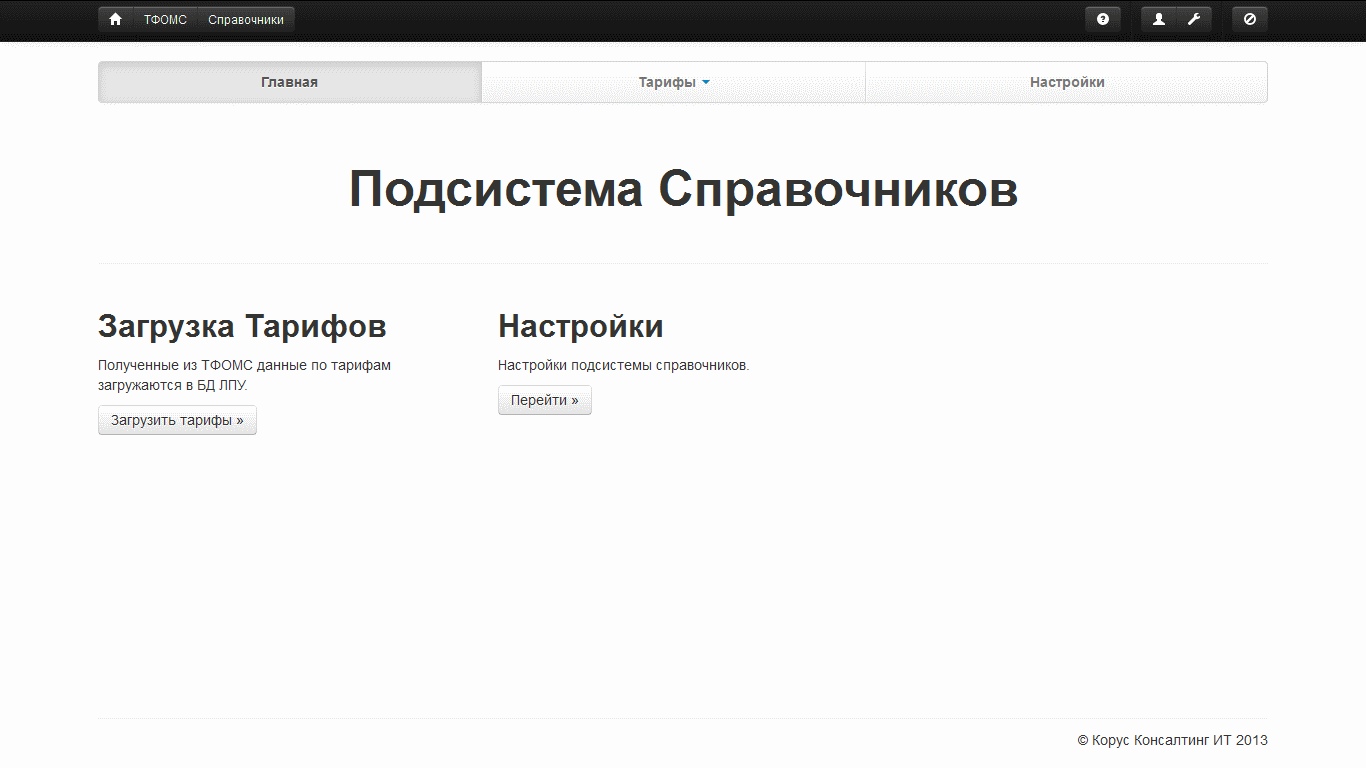
\includegraphics[width = 1\textwidth ,keepaspectratio]{spr_main}
 \caption{Главная страница подсистемы справочников}
 \label{img_spr_main}
\end{figure}

\subsection{Загрузка тарифов}

В данном разделе подсистемы осуществляется загрузка справочника тарифов по оплате услуг ЛПУ.

Для перехода в данный раздел (Рисунок \ref{img_spr_load}) необходимо нажать кнопку \btn{Тарифы}  в верхней части любой страницы подсистемы и в появившемся меню выбрать пункт Загрузка, либо нажать кнопку \btn{Загрузить тарифы >>} на главной странице подсистемы.

\begin{figure}[ht]\centering
 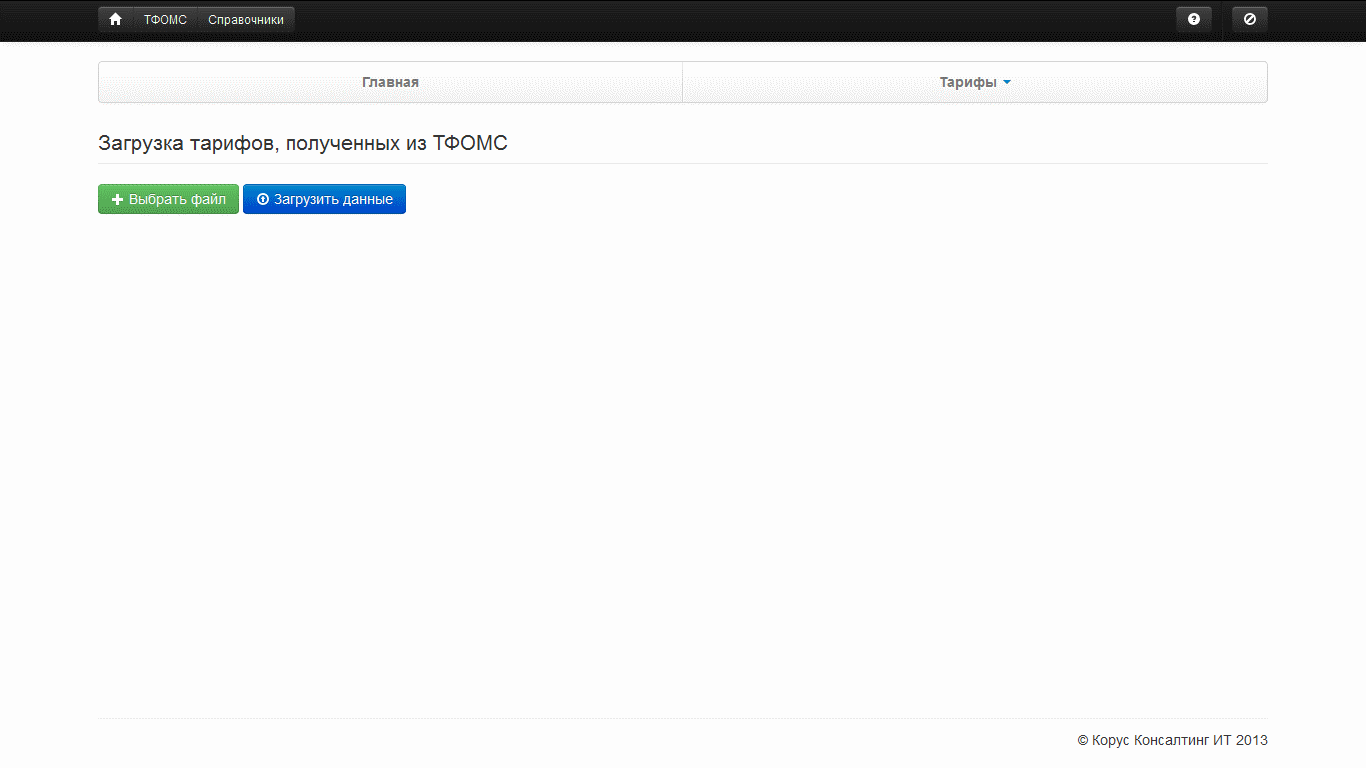
\includegraphics[width = 1\textwidth ,keepaspectratio]{spr_load}
 \caption{Страница загрузки справочника тарифов}
 \label{img_spr_load}
\end{figure}

Для загрузки тарифов необходимо нажать на кнопку \btn{Выбрать файл}, в открывшемся окне перейти в нужную папку и выбрать файл для загрузки. После выбора файла его имя появится под кнопкой \btn{Выбрать файл}. Далее необходимо нажать кнопку  \btn{Загрузить данные}. После некоторого времени ожидания на странице появится сообщение о результатах загрузки (Рисунок \ref{img_spr_load_rez}).

\begin{figure}[ht]\centering
 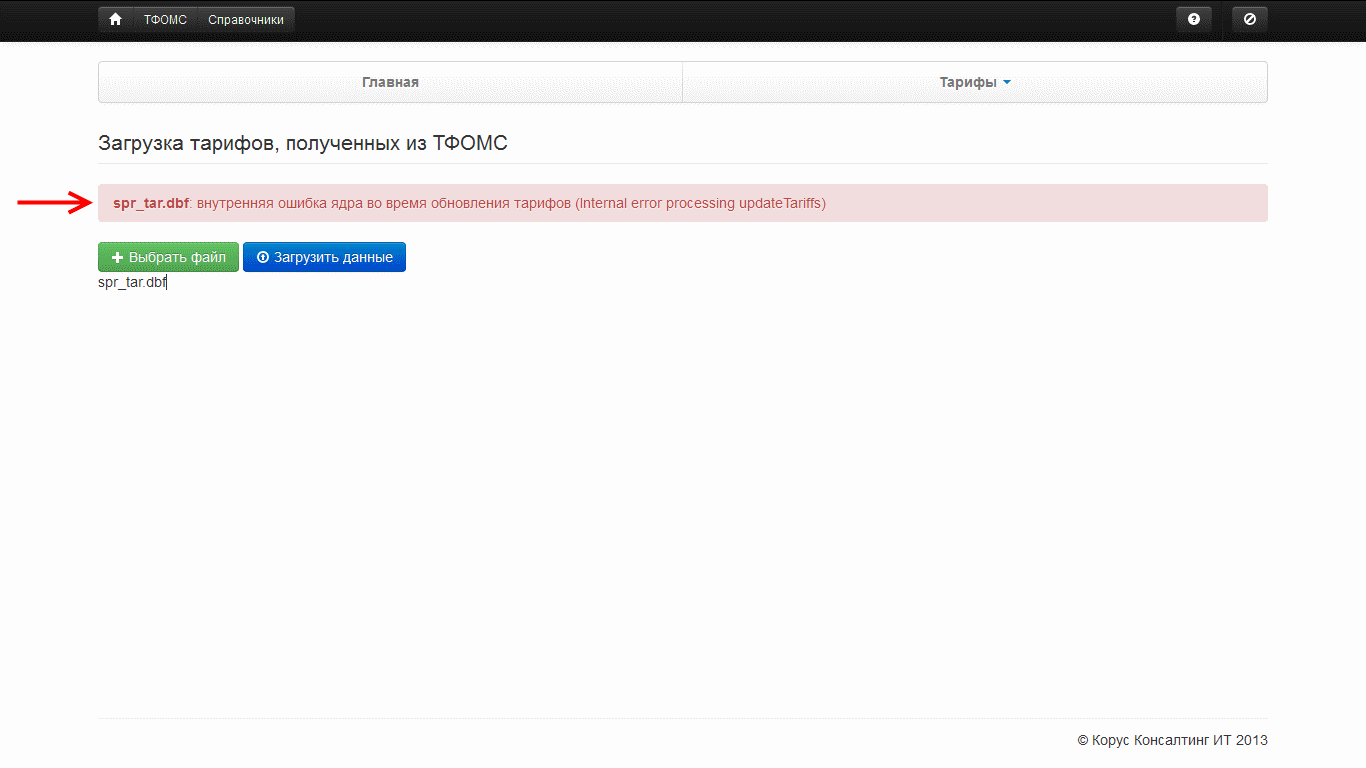
\includegraphics[width = 1\textwidth ,keepaspectratio]{spr_load_rez}
 \caption{Результат загрузки тарифов}
 \label{img_spr_load_rez}
\end{figure} %Подсистема справочников
 \end{document}